\documentclass[../main]{subfiles}

\graphicspath{{../figures/}}

\begin{document}

\section{提案手法のコンセプト}
\label{sec:pmethod_concept}
従来手法では異常音の抽出にヒューリスティックに設計したフィルタリングを用いるため,多様な異常音に対応することがができなかったり,空間的に離散的なモデルを用いているため,異常の位置特定が困難であった.

本研究では,これらの課題の解決を目的とし,以下のアプローチを採用する.
第一に,正常音を予測し,異常音を予測した正常音と観測音との差としてとらえることで,異常音に関する事前知識を必要とせず,汎用的に異常音を抽出する.
第二に,各地点での異常音の大きさを関連付け,これらの情報と音の大きさが空間的に減衰する性質を基に異常の発生場所を特定する.


次にこれらのアプローチを実現するための提案手法について述べる.
具体的には,移動ロボットが正常状態で記録した音のデータを用い,各座標とその地点での正常音との関係性を学習するモデルをニューラルネットワークを用いて構築する.
このモデルは,経路に沿った座標における正常音を予測することができ,観測された音との比較によってその地点で聞こえる異常音を検出する.
更に,異常音を検出した各地点の異常音の大きさを関連付けることで,異常音の発生場所を特定する.

これらの提案手法の背景には,現場作業員が異常音を検出する際のプロセスがある.
人間は,数回の点検を通じて各地点での正常音を脳内に記憶し,観測された音と正常音を比較することで異常を検出する.
また,異常音源の位置を特定する際には,空間的に動き回りながら,各地点での異常音の大きさを相対的に評価する.
本研究では,この人間のプロセスを模倣しつつ,移動ロボットと音響データを組み合わせることで,異常音の教師データを必要としない,
異常の検出と位置特定を実現する.

提案手法のフローチャートを図\ref{fig:flowchart}に示す.


\begin{figure}[t]
  \centering
  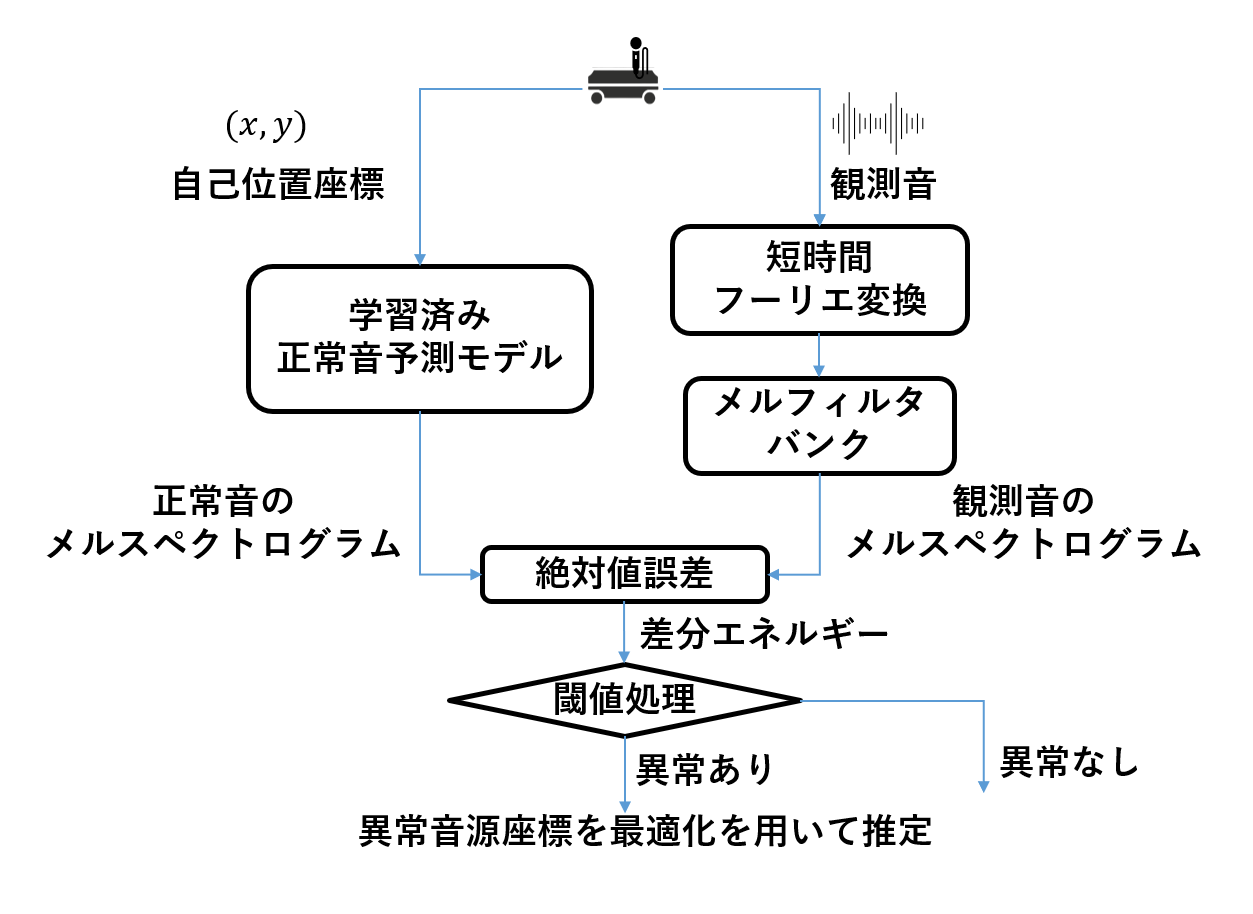
\includegraphics[keepaspectratio, width=1.0\linewidth]{chap3/flowchart_proposed_method.png}
  \caption{提案手法のフローチャート}
  \label{fig:flowchart}
\end{figure}

\end{document}
